\documentclass[aspectratio=169,10pt]{beamer}

% ==========================================================
% v2.tex — invited talk deck (TU/e 30 min, TUM 60 min)
% Single narrative thesis:
%   Scheduling in business processes is fundamentally non-local.
% Toggle:
%   \longfalse  -> TU/e (CORE + a single valuation intuition slide)
%   \longtrue   -> TUM (CORE + EXPAND + valuation climax)
% ==========================================================

% ---- Talk-length toggle ----
\newif\iflong
\longfalse      % TU/e (30 min)
% \longtrue     % TUM (60 min)

% ---- Theme ----
\usetheme{Madrid}
\usecolortheme{beaver}
\setbeamertemplate{navigation symbols}{}
\setbeamertemplate{footline}[frame number]
\setbeamerfont{title}{series=\bfseries}
\setbeamerfont{frametitle}{series=\bfseries}

% ---- Packages ----
\usepackage[T1]{fontenc}
\usepackage[utf8]{inputenc}
\usepackage{graphicx}
\usepackage{booktabs}
\usepackage{amsmath,amssymb}
\usepackage{mathtools}
\usepackage{xcolor}
\usepackage{tikz}
\usetikzlibrary{arrows.meta,positioning,shapes.geometric,calc,fit}

% ---- Figures in repo ----
\graphicspath{
  {Business_Process_Optimization/figs/}
  {ICAPS_problem_definition_final/images/}
  {IJCAI2026_Learn_to_Schedule/}
  {IJCAI2026_Learn_to_Schedule/new_plot/}
}

% ---- Helpers ----
\definecolor{darkred}{RGB}{140,0,0}
\definecolor{darkgray}{RGB}{60,60,60}
\definecolor{okblue}{RGB}{31,119,180}
\definecolor{okgreen}{RGB}{44,160,44}
\definecolor{okorange}{RGB}{255,127,14}
\definecolor{badred}{RGB}{214,39,40}
\newcommand{\btext}[1]{\textbf{\color{darkred}#1}}

% ---- Section slide (claim-style) ----
\AtBeginSection[]{
  \begin{frame}{The case against locality is cumulative}
    \tableofcontents[currentsection,hideothersubsections]
  \end{frame}
}

% ==========================================================
% Title
% ==========================================================
\title[Structure-Aware BPO Scheduling]{Structure-Aware Scheduling in Business Processes:\\Why Local Rules Fail and What Replaces Them}
\author[Arik Senderovich]{Arik Senderovich}
\institute[York University]{York University}
\date{January 2026}

\begin{document}

% CORE
\begin{frame}
  \titlepage
  \vspace{-0.25cm}
  \begin{center}\small\color{darkgray}
    \iflong
      Technical University of Munich
    \else
      Eindhoven University of Technology
    \fi
  \end{center}
\end{frame}

% CORE
\begin{frame}{Scheduling in business processes is fundamentally non-local}
  \begin{block}{Dominant thesis}
    Local dispatching rules, naive learning objectives, and ``fair'' heuristics fail once
    \btext{uncertainty}, \btext{downstream costs}, and \btext{synchronization} are present.
    \vspace{0.15cm}

    \btext{Structure-aware} optimization and \btext{valuation} are necessary.
  \end{block}

  \vspace{0.2cm}
  \begin{center}
    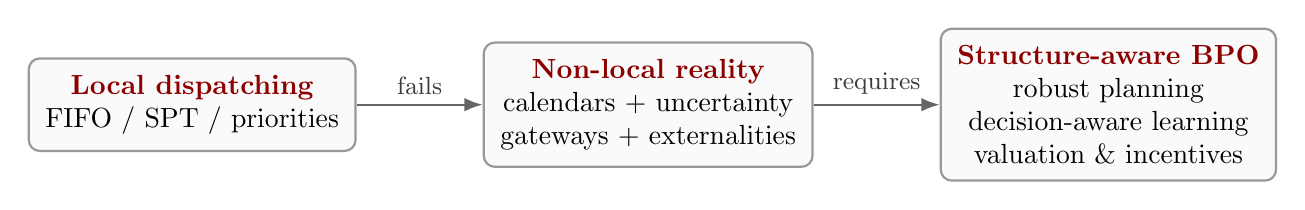
\begin{tikzpicture}[
      node distance=1.2cm and 1.6cm,
      box/.style={rounded corners, draw=black!40, thick, fill=black!2, inner sep=6pt, align=center},
      arr/.style={-Latex, thick, draw=black!60}
    ]
      \node[box] (local) {\btext{Local dispatching}\\FIFO / SPT / priorities};
      \node[box, right=of local] (nonlocal) {\btext{Non-local reality}\\calendars + uncertainty\\gateways + externalities};
      \node[box, right=of nonlocal] (fix) {\btext{Structure-aware BPO}\\robust planning\\decision-aware learning\\valuation \& incentives};
      \draw[arr] (local) -- node[above, font=\small, color=darkgray]{fails} (nonlocal);
      \draw[arr] (nonlocal) -- node[above, font=\small, color=darkgray]{requires} (fix);
    \end{tikzpicture}
  \end{center}
\end{frame}

% ==========================================================
% 1) BPO as high-stakes decision making
% ==========================================================
\section{BPO as high-stakes decision making}

% CORE
\begin{frame}{BPO turns process models into operational commitments}
  \begin{center}
    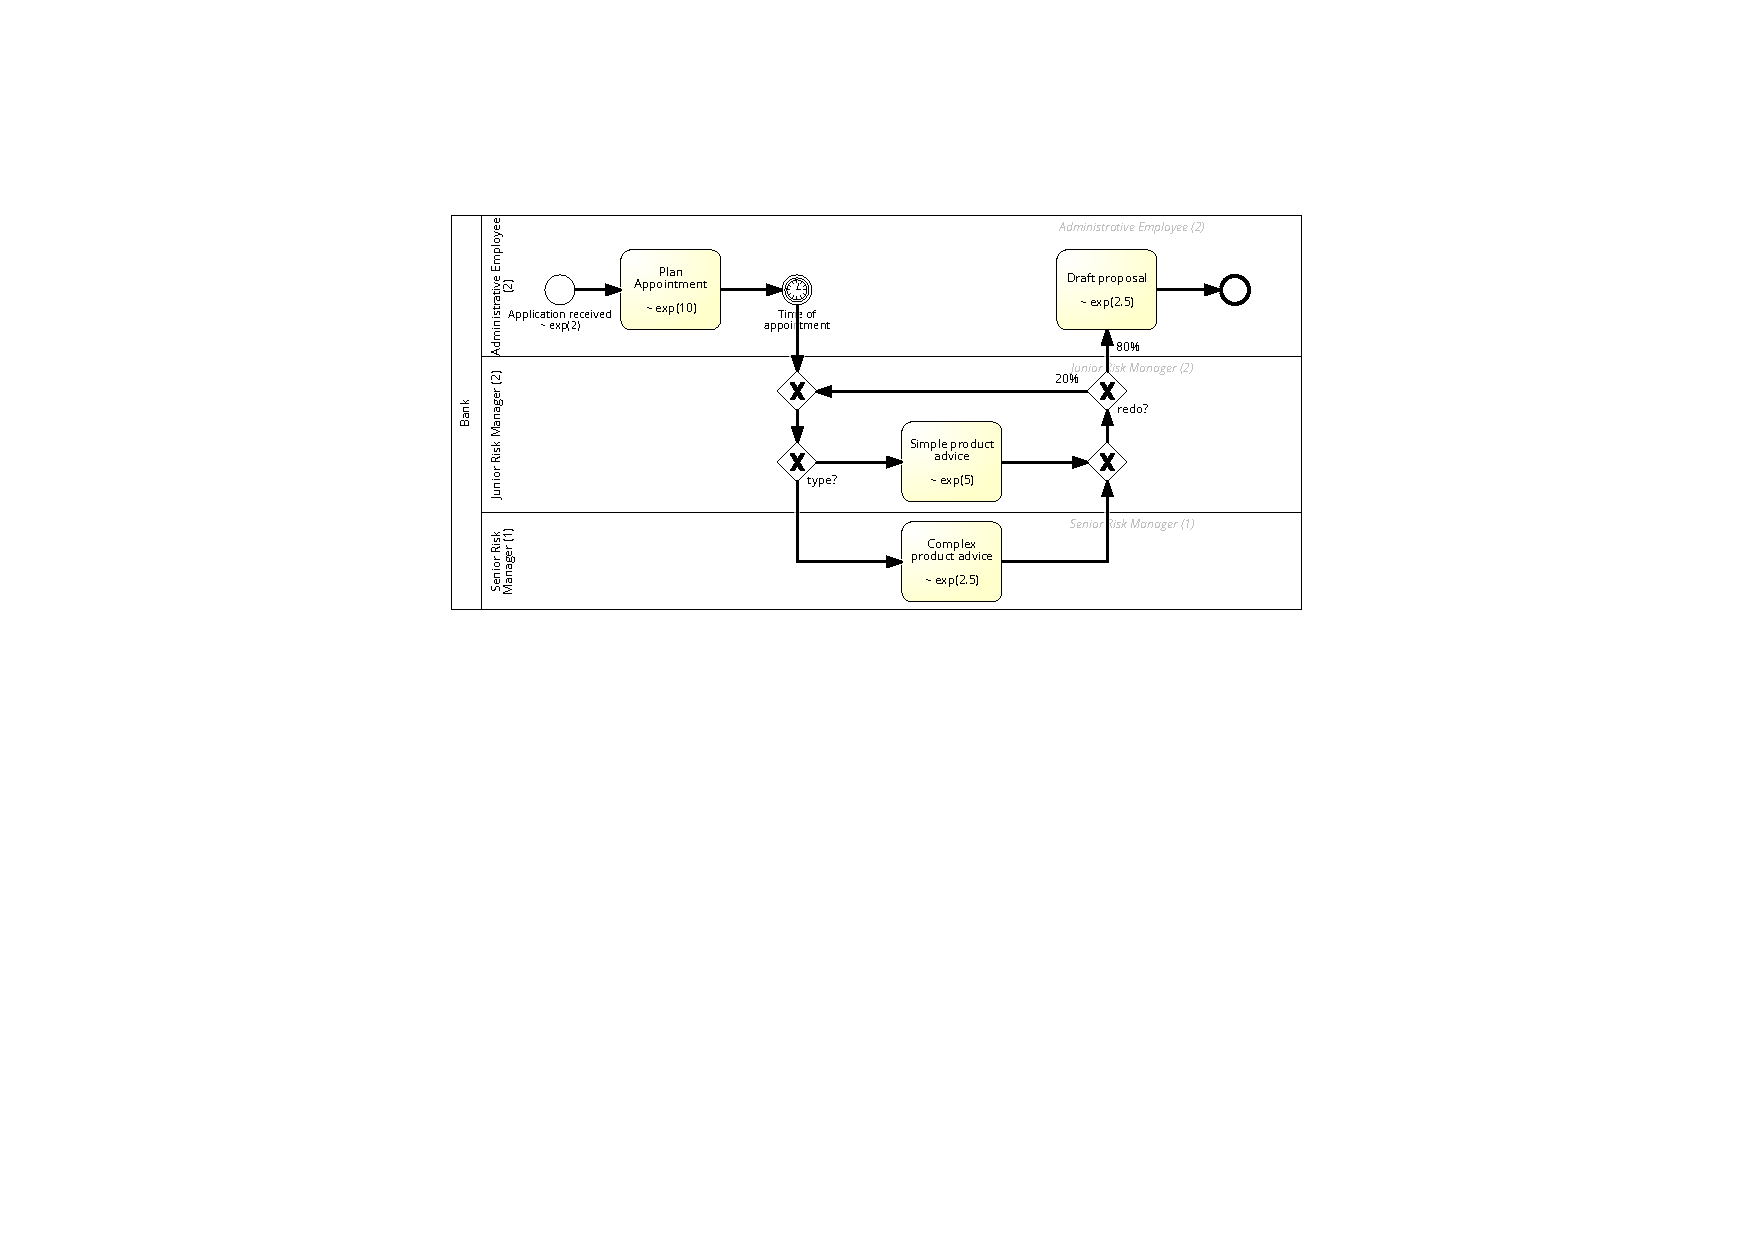
\includegraphics[width=0.98\textwidth,height=0.78\textheight,keepaspectratio]{process.pdf}
  \end{center}
  \vspace{-0.15cm}
  \scriptsize\color{darkgray}
  One BPMN model already implies nontrivial operational decisions (admission, routing, prioritization, staffing).
\end{frame}

% CORE
\begin{frame}{DayHospital is the archetype: high volume, high variability, high stakes}
  \begin{columns}[T]
    \column{0.62\textwidth}
      \begin{itemize}
        \item \btext{Many patients, many activities, many resources}
        \item \btext{Calendars}: shifts, partial capacity, vacations
        \item \btext{Uncertainty}: human-driven durations with heavy tails
        \item \btext{Outcome matters}: congestion and completion time
      \end{itemize}
      \vspace{0.25cm}
      \begin{block}{A single story, multiple failure modes}
        The same setting exposes three non-locality mechanisms:
        \btext{robustness}, \btext{optimization mismatch}, \btext{synchronization externalities}.
      \end{block}

    \column{0.38\textwidth}
      \centering
      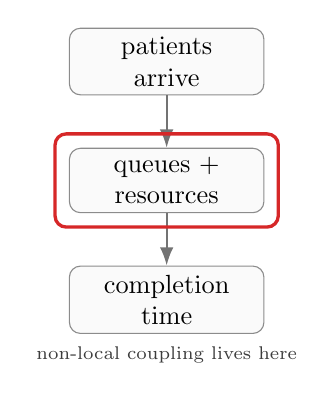
\begin{tikzpicture}[
        scale=0.95, every node/.style={transform shape},
        q/.style={rounded corners, draw=black!45, fill=black!2, minimum width=2.6cm, minimum height=0.75cm, align=center},
        arr/.style={-Latex, thick, draw=black!55}
      ]
        \node[q] (arrive) {patients\\arrive};
        \node[q, below=0.7cm of arrive] (queues) {queues +\\resources};
        \node[q, below=0.7cm of queues] (complete) {completion\\time};
        \draw[arr] (arrive) -- (queues);
        \draw[arr] (queues) -- (complete);
        \node[draw=badred, very thick, rounded corners, fit=(queues), inner sep=5pt] {};
        \node[below=0.05cm of complete, font=\scriptsize, color=darkgray] {non-local coupling lives here};
      \end{tikzpicture}
  \end{columns}
\end{frame}

% CORE
\begin{frame}{``Just dispatch'' fails because it ignores downstream consequences}
  \begin{block}{Local rule}
    Decide based on the \emph{current} queue only (FIFO / SPT / static priorities).
  \end{block}
  \vspace{0.1cm}
  \begin{block}{Reality in business processes}
    \begin{itemize}
      \item calendars couple decisions across time
      \item uncertainty couples decisions across scenarios
      \item gateways couple decisions across branches and cases
    \end{itemize}
  \end{block}
  \vspace{0.15cm}
  \btext{Claim:} locality is the wrong abstraction for BPO scheduling.
\end{frame}

% ==========================================================
% 2) Why local rules fail
% ==========================================================
\section{Why local rules fail in business processes}

% CORE
\begin{frame}{Three mechanisms break locality in BPO scheduling}
  \begin{center}
    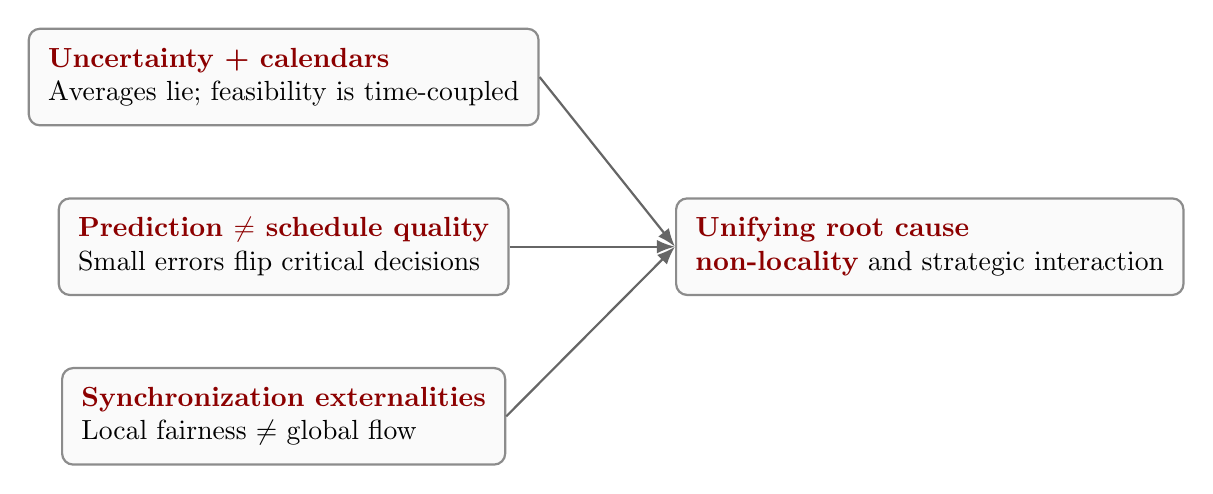
\begin{tikzpicture}[
      node distance=0.9cm and 1.6cm,
      box/.style={rounded corners, draw=black!45, thick, fill=black!2, inner sep=7pt, align=left},
      arr/.style={-Latex, thick, draw=black!60}
    ]
      \node[box] (u) {{\bfseries\color{darkred}Uncertainty + calendars}\\Averages lie; feasibility is time-coupled};
      \node[box, below=of u] (m) {{\bfseries\color{darkred}Prediction \(\neq\) schedule quality}\\Small errors flip critical decisions};
      \node[box, below=of m] (s) {{\bfseries\color{darkred}Synchronization externalities}\\Local fairness \(\neq\) global flow};
      \node[box, right=2.1cm of m] (th) {{\bfseries\color{darkred}Unifying root cause}\\\btext{non-locality} and strategic interaction};
      \draw[arr] (u.east) -- (th.west);
      \draw[arr] (m.east) -- (th.west);
      \draw[arr] (s.east) -- (th.west);
    \end{tikzpicture}
  \end{center}
\end{frame}

% ==========================================================
% 3) BPSP — handling uncertainty
% ==========================================================
\section{Robust proactive scheduling makes uncertainty operational (BPSP)}

% CORE
\begin{frame}{Averages lie when durations are stochastic and calendars bind}
  \begin{center}
    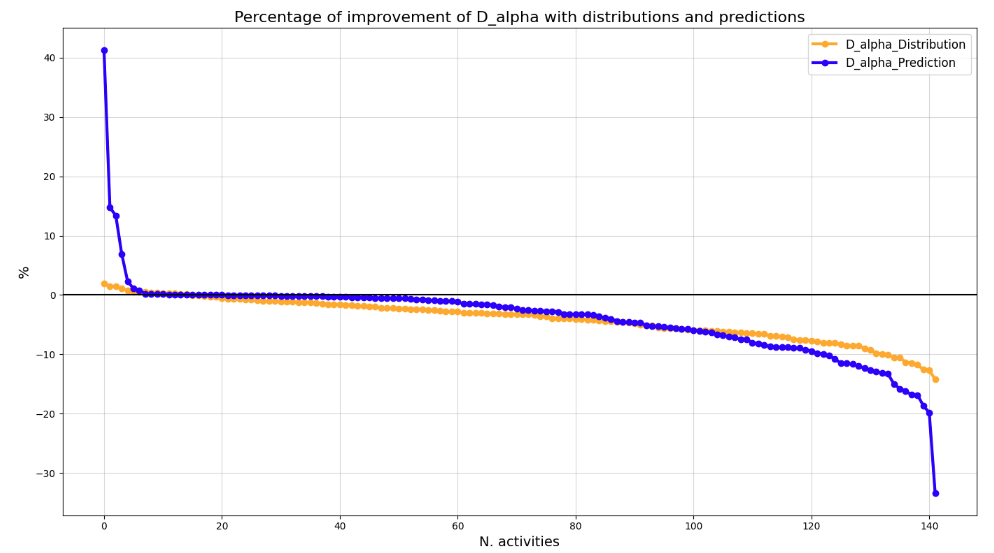
\includegraphics[width=0.95\textwidth,height=0.72\textheight,keepaspectratio]{distribution_predictions.png}
  \end{center}
  \vspace{-0.15cm}
  \scriptsize\color{darkgray}
  Logs reveal variability (\(\mu,\sigma\))—a single ``average duration'' is not a decision-relevant summary.
\end{frame}

% CORE — mandatory visual: Gantt with calendar blocking
\begin{frame}{Calendar blocking makes feasibility non-local in time}
  \begin{center}
    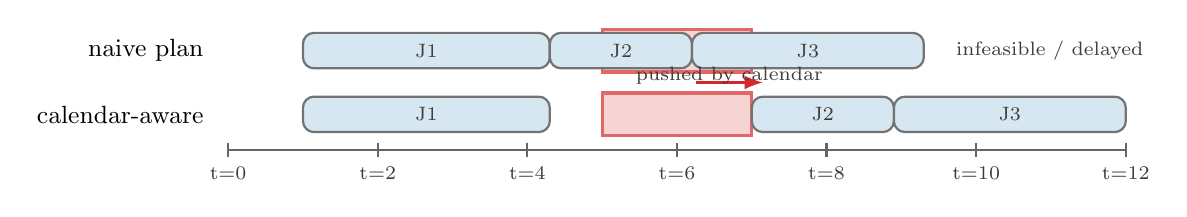
\begin{tikzpicture}[
      x=0.95cm, y=0.9cm,
      job/.style={rounded corners, draw=black!55, thick, fill=okblue!18, minimum height=0.55cm},
      vac/.style={draw=badred!70, very thick, fill=badred!20},
      axis/.style={draw=black!60, thick},
      lab/.style={font=\small},
      tiny/.style={font=\scriptsize, color=darkgray}
    ]
      % timeline
      \draw[axis] (0,0) -- (12,0);
      \foreach \t in {0,2,4,6,8,10,12} {
        \draw[axis] (\t,0.1) -- (\t,-0.1);
        \node[tiny, below] at (\t, -0.1) {t=\t};
      }

      % row labels
      \node[lab, anchor=east] at (-0.2, 1.4) {naive plan};
      \node[lab, anchor=east] at (-0.2, 0.5) {calendar-aware};

      % vacation block (shared)
      \draw[vac] (5.0,1.1) rectangle (7.0,1.7);
      \node[tiny] at (6.0,1.4) {vacation};
      \draw[vac] (5.0,0.2) rectangle (7.0,0.8);

      % naive plan jobs (would overlap vacation)
      \draw[job] (1.0,1.15) rectangle (4.3,1.65) node[midway,tiny]{J1};
      \draw[job] (4.3,1.15) rectangle (6.2,1.65) node[midway,tiny]{J2};
      \draw[job] (6.2,1.15) rectangle (9.3,1.65) node[midway,tiny]{J3};
      \node[tiny, anchor=west] at (9.6,1.4) {infeasible / delayed};

      % calendar-aware plan jobs (shifted right)
      \draw[job] (1.0,0.25) rectangle (4.3,0.75) node[midway,tiny]{J1};
      \draw[job] (7.0,0.25) rectangle (8.9,0.75) node[midway,tiny]{J2};
      \draw[job] (8.9,0.25) rectangle (12.0,0.75) node[midway,tiny]{J3};
      \draw[-Latex, thick, draw=badred] (6.25,0.95) -- (7.15,0.95);
      \node[tiny] at (6.7,1.05) {pushed by calendar};
    \end{tikzpicture}
  \end{center}
  \vspace{-0.1cm}
  \scriptsize\color{darkgray}
  A local decision at \(t=4\) is constrained by a calendar event at \(t\in[5,7]\).
\end{frame}

% CORE
\begin{frame}{Robust proactive scheduling converts logs into actionable plans}
  \begin{center}
    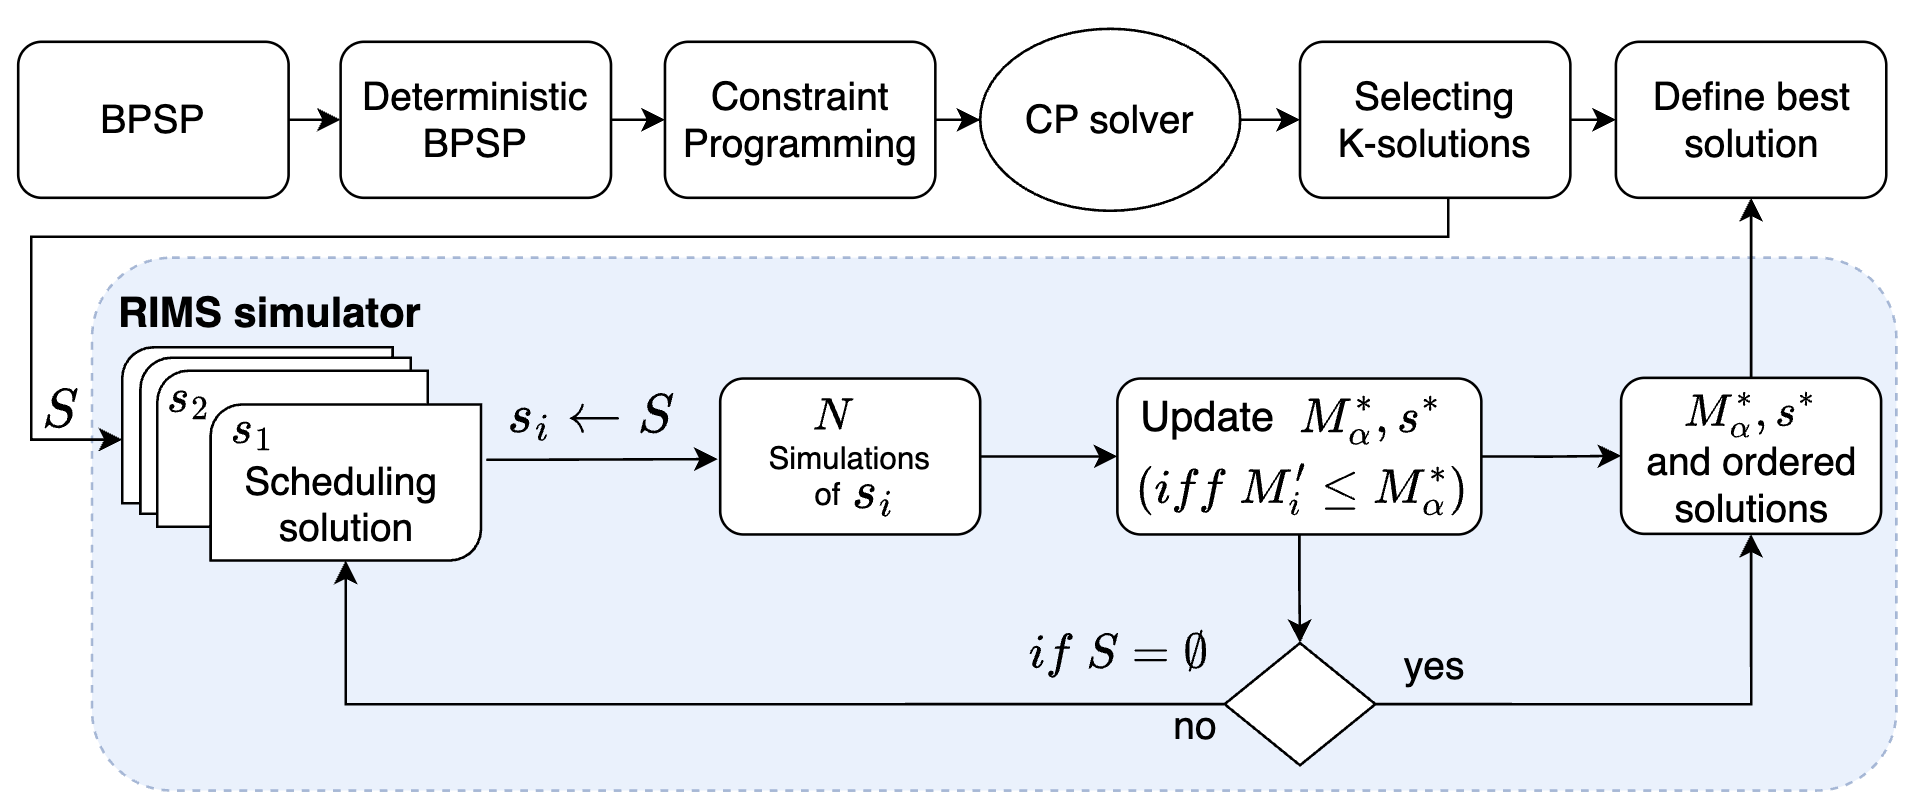
\includegraphics[width=0.98\textwidth,height=0.78\textheight,keepaspectratio]{pipeline_rims3.png}
  \end{center}
  \vspace{-0.15cm}
  \scriptsize\color{darkgray}
  Event logs \(\rightarrow\) uncertainty model \(\rightarrow\) CP schedules \(\rightarrow\) simulation-based selection.
\end{frame}

% CORE
\begin{frame}{Proactive schedules reduce makespan in DayHospital}
  \begin{block}{Outcome}
    Robust proactive scheduling improves makespan by \btext{5--14\%} on real hospital days.
  \end{block}
  \vspace{0.2cm}
  \begin{center}
    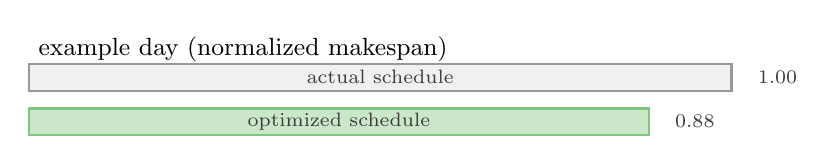
\begin{tikzpicture}[
      x=1.05cm, y=0.75cm,
      bar/.style={fill=okgreen!25, draw=okgreen!60, thick},
      base/.style={fill=black!6, draw=black!40, thick},
      tiny/.style={font=\scriptsize, color=darkgray}
    ]
      \node[anchor=west] at (0,1.8) {\small example day (normalized makespan)};
      \draw[base] (0,1.1) rectangle (8.5,1.55);
      \node[tiny] at (4.25,1.33) {actual schedule};
      \draw[bar] (0,0.35) rectangle (7.5,0.8);
      \node[tiny] at (3.75,0.58) {optimized schedule};
      \node[tiny, anchor=west] at (8.7,1.33) {1.00};
      \node[tiny, anchor=west] at (7.7,0.58) {0.88};
    \end{tikzpicture}
  \end{center}
  \vspace{0.1cm}
  \btext{Takeaway:} uncertainty-aware + calendar-aware planning is a necessary first fix.
\end{frame}

% EXPAND — theorem kept light
\iflong
% EXPAND
\begin{frame}{A single guarantee explains why buffered planning is principled}
  \begin{block}{Informal theorem (proactive lower bound)}
    For confidence level \(1-\alpha\), choosing a buffer coefficient
    \[
      q_U=\frac{\Phi^{-1}(1-\alpha)}{\sqrt{U}}
    \]
    yields a deterministic schedule whose makespan lower-bounds the
    \((1-\alpha)\)-probabilistic makespan target.
  \end{block}
  \vspace{0.1cm}
  \begin{block}{Why calendars do not break the argument (intuition)}
    Planned unavailability can be represented as fixed ``dummy'' intervals that enforce precedence-like feasibility.
  \end{block}
\end{frame}
\fi

% ==========================================================
% 4) SASS — handling optimization mismatch
% ==========================================================
\section{Decision-aware learning fixes prediction--optimization mismatch (SASS)}

% CORE
\begin{frame}{Prediction accuracy is not scheduling performance}
  \begin{block}{Mismatch}
    Mean-squared error (MSE) optimizes numeric accuracy, but scheduling objectives depend on
    \btext{discrete decisions} (orderings, groupings, threshold tests).
  \end{block}
  \vspace{0.2cm}
  \btext{Claim:} in scheduling, small prediction errors can cause large regret.
\end{frame}

% CORE — mandatory visual: 2-job swap cartoon
\begin{frame}{A tiny prediction error can flip an ordering decision—and the cost is large}
  \begin{columns}[T]
    \column{0.52\textwidth}
      \btext{True durations:} \(y_A=10,\; y_B=11\) \\
      \btext{Optimal (SPT):} \(A \rightarrow B\)
      \vspace{0.25cm}

      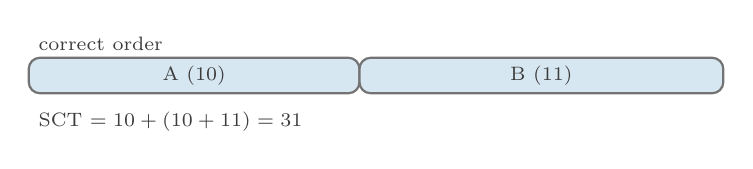
\begin{tikzpicture}[
        x=0.42cm, y=0.9cm,
        job/.style={rounded corners, draw=black!55, thick, fill=okblue!18, minimum height=0.55cm},
        tiny/.style={font=\scriptsize, color=darkgray}
      ]
        \node[tiny, anchor=west] at (0,1.05) {correct order};
        \draw[job] (0,0.35) rectangle (10,0.85) node[midway,tiny]{A (10)};
        \draw[job] (10,0.35) rectangle (21,0.85) node[midway,tiny]{B (11)};
        \node[tiny, anchor=west] at (0,-0.05) {SCT \(=10+(10+11)=31\)};
      \end{tikzpicture}

    \column{0.48\textwidth}
      \btext{Predicted:} \(\hat y_A=10.6,\; \hat y_B=10.5\) \\
      \btext{Chosen:} \(B \rightarrow A\)
      \vspace{0.25cm}

      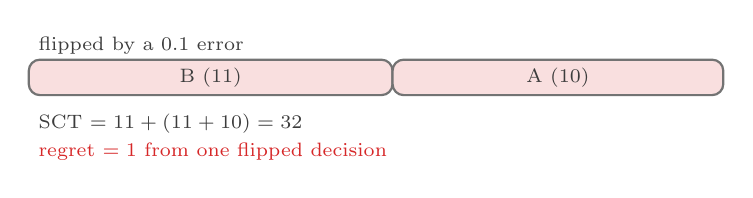
\begin{tikzpicture}[
        x=0.42cm, y=0.9cm,
        job/.style={rounded corners, draw=black!55, thick, fill=badred!15, minimum height=0.55cm},
        tiny/.style={font=\scriptsize, color=darkgray}
      ]
        \node[tiny, anchor=west] at (0,1.05) {flipped by a 0.1 error};
        \draw[job] (0,0.35) rectangle (11,0.85) node[midway,tiny]{B (11)};
        \draw[job] (11,0.35) rectangle (21,0.85) node[midway,tiny]{A (10)};
        \node[tiny, anchor=west] at (0,-0.05) {SCT \(=11+(11+10)=32\)};
        \node[tiny, anchor=west, color=badred] at (0,-0.45) {regret \(=1\) from one flipped decision};
      \end{tikzpicture}
  \end{columns}
\end{frame}

% CORE
\begin{frame}{SASS trains on the critical decisions that determine the schedule}
  \begin{center}
    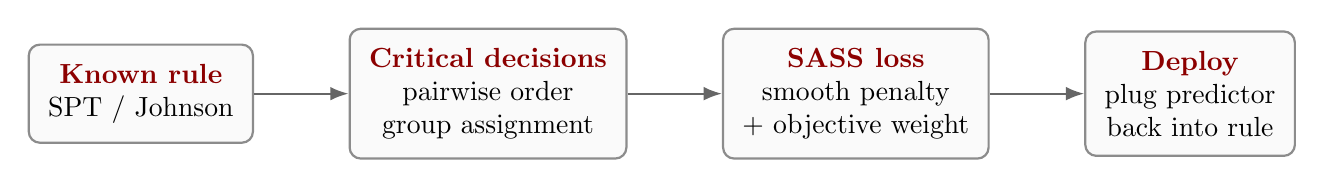
\begin{tikzpicture}[
      node distance=1.0cm and 1.2cm,
      box/.style={rounded corners, draw=black!45, thick, fill=black!2, inner sep=7pt, align=center},
      arr/.style={-Latex, thick, draw=black!60}
    ]
      \node[box] (rule) {\btext{Known rule}\\SPT / Johnson};
      \node[box, right=of rule] (dec) {\btext{Critical decisions}\\pairwise order\\group assignment};
      \node[box, right=of dec] (loss) {\btext{SASS loss}\\smooth penalty\\\(+\) objective weight};
      \node[box, right=of loss] (deploy) {\btext{Deploy}\\plug predictor\\back into rule};
      \draw[arr] (rule) -- (dec);
      \draw[arr] (dec) -- (loss);
      \draw[arr] (loss) -- (deploy);
    \end{tikzpicture}
  \end{center}
  \vspace{0.15cm}
  \btext{Claim:} learning becomes stable when it mirrors the algorithmic structure of scheduling.
\end{frame}

% EXPAND — synthetic evidence
\iflong
% EXPAND
\begin{frame}{SASS remains stable as noise increases (synthetic evidence)}
  \begin{center}
    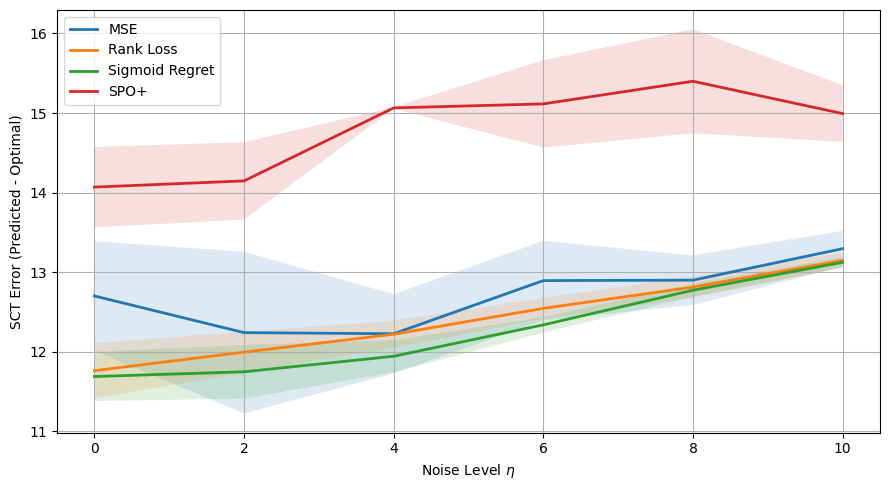
\includegraphics[width=0.95\textwidth,height=0.75\textheight,keepaspectratio]{linearDataset_problem1.png}
  \end{center}
  \vspace{-0.15cm}
  \scriptsize\color{darkgray}
  Relative SCT error vs.\ the optimal schedule under increasing noise (SASS vs baselines).
\end{frame}
\fi

% CORE — real-world headline, no placeholder
\begin{frame}{SASS improves schedules in the real clinic, not just predictions}
  \begin{columns}[T]
    \column{0.58\textwidth}
      \begin{block}{DayHospital outpatient sequencing (Jan--Dec 2021)}
        \begin{itemize}
          \item Objective: minimize congestion (SCT)
          \item Metric: average relative SCT error vs.\ optimal ordering
        \end{itemize}
      \end{block}

      \begin{table}
        \small
        \setlength{\tabcolsep}{6pt}
        \renewcommand{\arraystretch}{1.15}
        \begin{tabular}{l c}
          \toprule
          Method & Avg.\ rel.\ SCT error \\
          \midrule
          \btext{SASS} & \btext{0.316} \\
          MSE (predict-then-optimize) & 0.353 \\
          LTR & 0.338 \\
          SPO+ & 0.476 \\
          \bottomrule
        \end{tabular}
      \end{table}

    \column{0.42\textwidth}
      \centering
      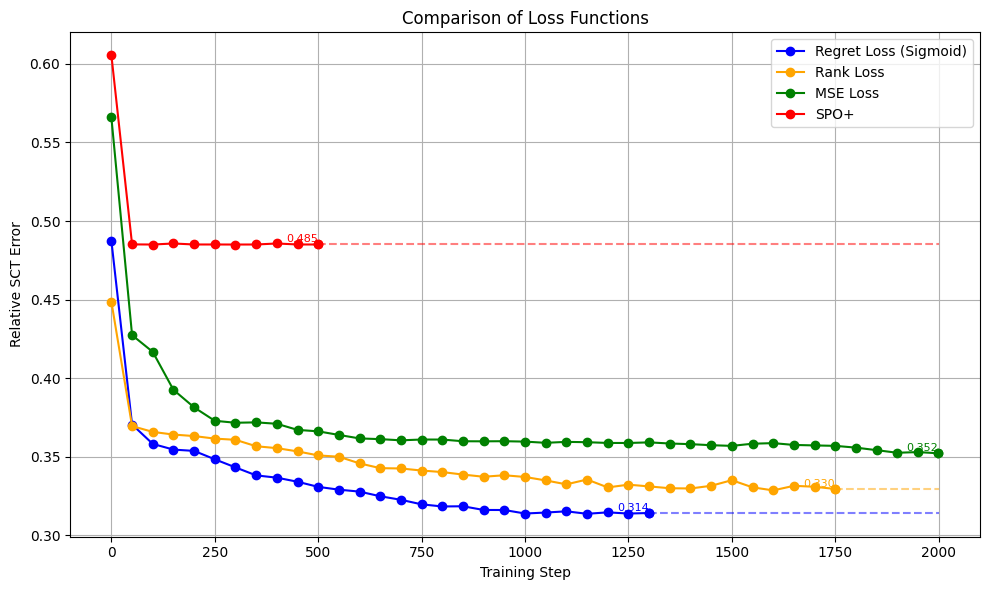
\includegraphics[width=0.95\textwidth,height=0.62\textheight,keepaspectratio]{LossComparison_Jan.png}
      \vspace{0.05cm}
      \scriptsize\color{darkgray}
      Training dynamics (Jan 2021).
  \end{columns}
\end{frame}

% ==========================================================
% 5) Why this is still not enough: synchronization & incentives
% ==========================================================
\section{Synchronization and incentives expose the last non-locality}

% CORE — required transition: SASS -> valuation
\begin{frame}{SASS assumes a single controller—real processes create strategic externalities}
  \begin{block}{Bridge}
    SASS optimizes a global objective for a single controller.
    \vspace{0.1cm}

    But in real workflows, \btext{cases optimize for themselves}, and synchronization creates
    \btext{delay externalities} across queues.
  \end{block}
  \vspace{0.2cm}
  \btext{Claim:} even perfect decision-aware learning is insufficient without a mechanism for externalities.
\end{frame}

% CORE — mandatory visual: OR-split example showing FIFO blocking fast branch
\begin{frame}{FIFO is locally fair but globally inefficient at OR joins}
  \begin{columns}[T]
    \column{0.55\textwidth}
      \centering
      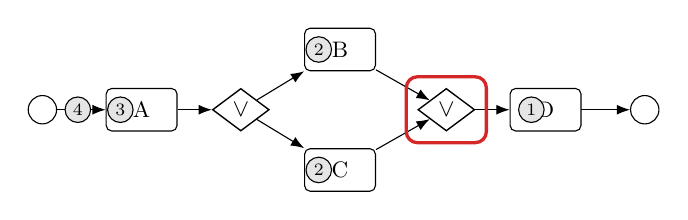
\begin{tikzpicture}[
        scale=0.9, every node/.style={transform shape},
        >=Latex,
        event/.style={circle,draw,minimum size=4mm},
        gateway/.style={diamond,draw,aspect=2.4,minimum width=8mm,minimum height=6mm,inner sep=0pt,line width=0.5pt},
        activity/.style={rectangle,draw,rounded corners=2pt,minimum width=10mm,minimum height=6mm,font=\small},
        case/.style={circle,draw,fill=black!10,inner sep=0.5pt,minimum size=3.6mm,font=\scriptsize}
      ]
        \node[event]    (start) at (0,0) {};
        \node[activity] (A)     at (1.4,0) {A};
        \node[gateway]  (split) at (2.8,0) {};
        \node[activity] (B)     at (4.2,0.85) {B};
        \node[activity] (C)     at (4.2,-0.85) {C};
        \node[gateway]  (join)  at (5.7,0) {};
        \node[activity] (D)     at (7.1,0) {D};
        \node[event]    (end)   at (8.5,0) {};

        \node at (split.center) {$\vee$};
        \node at (join.center)  {$\vee$};

        \draw[->] (start) -- (A);
        \draw[->] (A) -- (split);
        \draw[->] (split) -- (B);
        \draw[->] (split) -- (C);
        \draw[->] (B) -- (join);
        \draw[->] (C) -- (join);
        \draw[->] (join) -- (D);
        \draw[->] (D) -- (end);

        % cases: 1&2 need both; 3 needs B; 4 needs C
        \node[case] at (6.9, 0.00) {1};
        \node[case] at (3.9, 0.85) {2};
        \node[case] at (3.9,-0.85) {2};
        \node[case] at (1.1, 0.00) {3};
        \node[case] at (0.5, 0.00) {4};

        % highlight join
        \node[draw=badred, very thick, rounded corners, fit=(join), inner sep=4pt] {};
      \end{tikzpicture}
      \vspace{0.05cm}
      \scriptsize\color{darkgray}
      OR join couples queues \(B\) and \(C\).

    \column{0.45\textwidth}
      \begin{block}{What FIFO misses}
        \begin{itemize}
          \item Scheduling at \(B\) delays completion at \(C\), and vice versa.
          \item A locally fair order can create avoidable waiting at the join.
        \end{itemize}
      \end{block}
      \btext{Claim:} synchronization makes delay costs \emph{non-local} across branches.
  \end{columns}
\end{frame}

% For TU/e we stop valuation here (one intuition slide).
\iflong\else
% CORE
\begin{frame}{The missing ingredient is a signal for non-local delay costs}
  \begin{block}{One-sentence conclusion}
    Robust planning and decision-aware learning still assume a centralized controller;
    synchronization requires \btext{pricing} the externalities that cases impose on one another.
  \end{block}
  \vspace{0.2cm}
  \btext{Next:} valuation-aware scheduling (the TUM version’s climax).
\end{frame}
\fi

% ==========================================================
% 6) Valuation-aware scheduling (climax)
% ==========================================================
\iflong
\section{Valuation-aware scheduling is the conceptual capstone}

% EXPAND
\begin{frame}{Value-of-time reports make non-local costs explicit}
  \begin{columns}[T]
    \column{0.55\textwidth}
      \begin{block}{Interface}
        Each case reports a \btext{value-of-time} function: marginal cost of waiting over time.
      \end{block}
      \vspace{0.15cm}
      \begin{block}{Meaning}
        This compact signal implicitly encodes preferences over coordinated progress across multiple queues.
      \end{block}

    \column{0.45\textwidth}
      \centering
      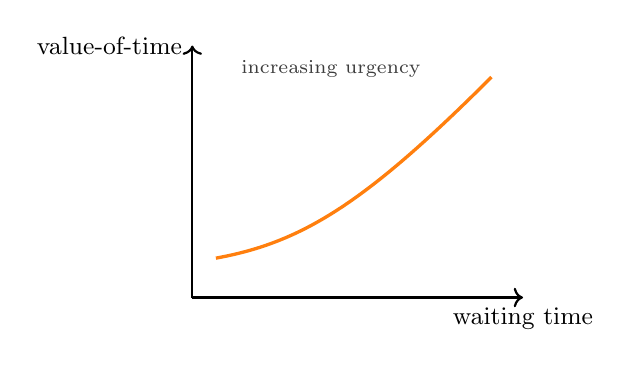
\begin{tikzpicture}[x=1.0cm,y=1.0cm]
        \draw[->, thick] (0,0) -- (4.2,0) node[below, font=\small]{waiting time};
        \draw[->, thick] (0,0) -- (0,3.2) node[left, font=\small]{value-of-time};
        \draw[very thick, color=okorange] (0.3,0.5) .. controls (1.4,0.7) and (2.2,1.2) .. (3.8,2.8);
        \node[font=\scriptsize, color=darkgray, anchor=west] at (0.5,2.9) {increasing urgency};
      \end{tikzpicture}
  \end{columns}
\end{frame}

% EXPAND
\begin{frame}{Pricing externalities reconciles efficiency and neutrality}
  \begin{block}{Principle}
    Deviations from FIFO are not ``unfair'' when they are accompanied by payments that
    exactly price the delay externalities imposed on others.
  \end{block}
  \vspace{0.15cm}
  \begin{center}
    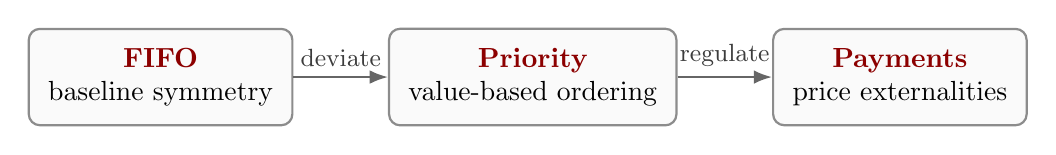
\begin{tikzpicture}[
      node distance=1.1cm and 1.2cm,
      box/.style={rounded corners, draw=black!45, thick, fill=black!2, inner sep=7pt, align=center},
      arr/.style={-Latex, thick, draw=black!60}
    ]
      \node[box] (fifo) {\btext{FIFO}\\baseline symmetry};
      \node[box, right=of fifo] (prio) {\btext{Priority}\\value-based ordering};
      \node[box, right=of prio] (vcg) {\btext{Payments}\\price externalities};
      \draw[arr] (fifo) -- node[above, font=\small, color=darkgray]{deviate} (prio);
      \draw[arr] (prio) -- node[above, font=\small, color=darkgray]{regulate} (vcg);
    \end{tikzpicture}
  \end{center}
  \vspace{0.1cm}
  \scriptsize\color{darkgray}
  VCG-style pricing yields truthful reporting in the valuation model.
\end{frame}

% EXPAND
\begin{frame}{Valuation is the unifier: it generalizes what BPSP and SASS cannot express}
  \begin{itemize}
    \item \btext{BPSP} handles uncertainty and calendars for a centralized planner.
    \item \btext{SASS} aligns learning with a planner’s objective under a known rule.
    \item \btext{Valuation} handles strategic cases and synchronization by making non-local costs explicit.
  \end{itemize}
  \vspace{0.2cm}
  \begin{block}{Climax}
    Non-locality is not an edge case—it is the defining feature of scheduling in business processes.
  \end{block}
\end{frame}
\fi

% ==========================================================
% 7) Synthesis & agenda
% ==========================================================
\section{Synthesis: Structure-aware BPO}

% CORE
\begin{frame}{Structure-aware BPO is a pipeline: logs \(\rightarrow\) learning \(\rightarrow\) incentives}
  \begin{center}
    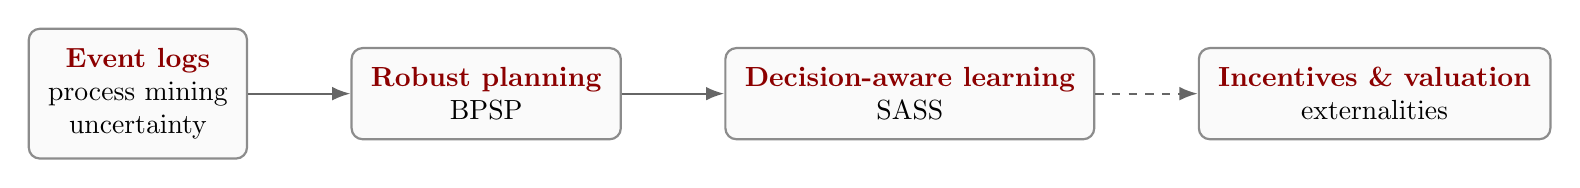
\begin{tikzpicture}[
      node distance=1.0cm and 1.3cm,
      box/.style={rounded corners, draw=black!45, thick, fill=black!2, inner sep=7pt, align=center},
      arr/.style={-Latex, thick, draw=black!60}
    ]
      \node[box] (logs) {\btext{Event logs}\\process mining\\uncertainty};
      \node[box, right=of logs] (rob) {\btext{Robust planning}\\BPSP};
      \node[box, right=of rob] (learn) {\btext{Decision-aware learning}\\SASS};
      \node[box, right=of learn] (inc) {\btext{Incentives \& valuation}\\externalities};
      \draw[arr] (logs) -- (rob);
      \draw[arr] (rob) -- (learn);
      \iflong
        \draw[arr] (learn) -- (inc);
      \else
        \draw[arr, dashed] (learn) -- (inc);
      \fi
    \end{tikzpicture}
  \end{center}
  \vspace{0.1cm}
  \btext{Claim:} the next generation of BPO is structure-aware end-to-end.
\end{frame}

% CORE
\begin{frame}{Take-home message: locality is the wrong default in business process scheduling}
  \begin{enumerate}
    \item \btext{Non-locality is structural}: calendars, uncertainty, gateways.
    \item \btext{Robust planning is necessary}: it makes uncertainty operational.
    \item \btext{Decision-aware learning is necessary}: it aligns training with schedule quality.
    \item \iflong\btext{Valuation is the capstone}: it prices externalities and enables neutrality with efficiency.\else\btext{Valuation is the next step}: it prices externalities created by synchronization.\fi
  \end{enumerate}
  \vspace{0.25cm}
  \btext{Thank you.}
\end{frame}

% ==========================================================
% Appendix
% ==========================================================
\appendix
\section{Appendix}

% APPENDIX
\begin{frame}{Buffered durations connect confidence to deterministic planning}
  \begin{block}{Buffered duration}
    \(d=\mu+q\sigma\) with \(q\) chosen from a confidence level.
  \end{block}
  \vspace{0.15cm}
  \begin{block}{Typical choice}
    \(q_U=\Phi^{-1}(1-\alpha)/\sqrt{U}\), where \(U\) upper-bounds uncertain activities on the critical path.
  \end{block}
  \scriptsize\color{darkgray}
  The appendix keeps details out of the main narrative.
\end{frame}

\end{document}

